Le projet étant open-source et actif, il évolue sans cesse. La partie sur laquelle nous avons travaillé est relativement stable mais son utilisation peut varier dans le code. Nous allons voir la portée de l'utilisation de nanoXml, comment il est utilisé et enfin la solution apportée.

% -> Utilisation intensive de XML
% -> Philosophie de nanoXml et de DOM differente
% -> -> DOM : Tout est noeud
% -> -> NanoXml : Base sur les tags (elements)
\section{Nanoxml}
Comme nous avons pu le voir, IzPack utilise intensément des fichiers XML pour la génération d'installations.
En effet, les fichiers XML présentent l'avantage d'être lisible, écrivable a la main et traitables.
Pour traiter ces fichiers, une librairie a été utilisée, il s'agit de NanoXml.
\subsection{Le projet NanoXml}
NanoXml est une librairie java open-source de gestion de Xml.
Elle présente la particularité d'être légère (108Ko). 
Il est possible, grâce a cette librairie, d'écrire ou de parser des fichiers Xml.
Une fois le fichier parsé, on récupère en mémoire la structure de l'arbre Xml qui peut alors être exploité.
Le choix de cette librairie a été faite au commencement de Izpack a cause de sa taille.
En effet, il est important que le la partie installeur ne surcharge pas excessivement sur le logiciel à installer.

Cependant ce projet n'est plus mis à jour depuis 7 ans, et des bugs ont été découverts.
Entre temps, java a ajouté a sa JRE (depuis la version 1.4) tout ce qu'il faut pour gérer le xml.
Il devenait intéressant de remplacer NanoXml par Jaxp (Java API for XML Processing), la librairie fournie par la machine virtuelle.
\subsection{Les différents composants de NanoXml}
On trouve différents éléments dans NanoXml.
\subsubsection{StdXMLParser}
Le parser permet de créer un arbre logique représentant le fichier xml qui lui a été passé.
Il est systématiquement utilisé au moment de la lecture du fichier afin de récupérer l'arbre.
\subsubsection{StdXMLWriter}
Le XMLWriter permet d'écrire des fichiers XML.
Il reproduit, à partir d'un XMLElement, le fichier XML correspondant.
Il n'est utilisé que pour générer un xml temporaire lors de la compilation ou pour écrire le xml d'installation automatique.
\subsubsection{XMLElement}
Le XMLElement représente un élément logique du xml en mémoire. Par exemple :
\begin{lstlisting}[language=xml]
<root>
	<child>
		content
	</child>
</root>
\end{lstlisting}
En parsant un fichier contenant ce Xml, on obtient un XMLElement nommé root qui possède 1 enfant, \verb|child|. Son enfant est un XMLElement dont le contenu est ``content''.

L'arborescence du XML est donc réalisé par un ensemble de XMLElement.
L'interface de XMLElement permet de récupérer la liste des enfants, le contenu, rechercher un enfant par son nom, retirer un enfant, ajouter un enfant ou modifier le contenu.
Il s'agit de loin de la classe la plus utilisée de la librairie NanoXml dans Izpack.
En effet, on ne comptait pas moins de 499 utilisations au commencement de ce projet.
\subsection{Utilisation typique dans Izpack}
\subsubsection{Parse de fichier}
Le parse du fichier est exécuté pour récupérer le XML.
\begin{lstlisting}
StdXMLParser parser = new StdXMLParser();
parser.setBuilder(XMLBuilderFactory.createXMLBuilder());
parser.setReader(new StdXMLReader(in));
parser.setValidator(new NonValidator());
// We get the data
XMLElement data = (XMLElement) parser.parse();
\end{lstlisting}
Avec cet exemple, on crée les objets nécessaires au parse d'un fichier, et on récupère dans \verb|data| la racine de l'arborescence du xml chargé en mémoire.
\subsubsection{Écriture d'un xml}
\begin{lstlisting}
XMLWriter writer = new XMLWriter(out);
...
writer.write(xmlElement);
\end{lstlisting}
Le XMLWriter prend un OutputStream à sa contruction.
On peut donc écrire un Xml dans tout type de flux de sortie. 
Une fois le XMLWriter instancié, il suffit de lui passer le \verb|xmlElement| représentant la racine de l'arborescence que l'on veut écrire.
\subsubsection{Utilisation de XMLElement}
La manipulation d'un XMLElement se fait avec ses méthodes :
\begin{itemize}
	\item get/setAttribute pour gérer les attributs du noeud
	\item get/setContent pour gérer le contenu
	\item add/removeChild pour gérer les noeuds fils
	\item etc
\end{itemize}
Voici un exemple d'utilisation :
% TODO : avoir un exemple plus clair/concis
\begin{lstlisting}
XMLElement root;
//...
Iterator<XMLElement> iter = root.getChildrenNamed("parsable").iterator();
while (iter.hasNext())
{
	XMLElement p = iter.next();
	String target = requireAttribute(p, "targetfile");
	String type = p.getAttribute("type", "plain");
	//...
}
\end{lstlisting}
\section{Jaxp}
Jaxp, le processeur Xml de Sun, respecte les normes W3C.
Il y a deux manières d'exploiter les XML avec Jaxp, soit en utilisant le parseur SAX, soit en utilisant le parseur DOM.
\subsection{SAX}
SAX (Simple API for Xml) est une API pour parser les XML.
Cette API possède la particularité de procéder par évènement.
C'est à dire que le parser va lire le fichier ligne par ligne et envoyer un évènement pour chaque élément particulier qu'il rencontre.

Des évènements sont lancés des que le parse rencontre des commentaires, du texte, des éléments...
L'avantages de cette API est l'utilisation mémoire faible, puisque le xml n'est pas mis en mémoire mais lu et traité au fur et à mesure, il permet de traiter sans problème les fichiers importants.
En contrepartie, le traitement et la manipulation du xml est plus difficile.
\subsection{DOM}
L'interface DOM (Document Object Model) de Jaxp propose de mettre en mémoire le xml et offre une interaction basée sur des noeuds (node en anglais).
En DOM tout est noeud, les commentaires, le texte ou les éléments sont représentés par des noeuds.
Le xml est est représenté par une arborescence de noeuds.
Des sous-classes spécialisent ces noeuds comme \verb|Comment|, \verb|Element| ou \verb|Text|.

La manipulation des éléments du xml se fait grâce aux nodes.
Il est possible de récupérer le voisin d'une node, d'enlever ou d'ajouter un enfant et de récupérer ou de modifier le contenu.
%--------------------------------------------------------------------------
\section{Élaboration de la solution}
Notre travail a été de chercher une solution pour permettre de remplacer de NanoXml et de l'appliquer au projet.
Cependant, ils y avaient plusieurs problèmes à cela.
\subsection{Les différences entre Jaxp et NanoXml}
Comme nous avons vu précédemment, les deux API ne proposent pas la même approche pour le traitement des fichiers xml.
Nous avons choisi d'utiliser l'interface DOM vu que les avantages de SAX ne sont pas nécessaires et qu'il était peu concevable de traiter les XML avec SAX dans IzPack.
De plus, NanoXml et DOM ont une représentation similaire du xml.
Nous allons donc comparer l'interface DOM et NanoXml pour déterminer la meilleure approche a prendre.
\subsubsection{Manipulation du XML}
La principale différence vient de l'élément atomique : le noeud de DOM ne représente pas la même notion que l'élément de nanoXML.
Dès lors, la manipulation des voisins, enfants, etc doit être adapté.
\begin{lstlisting}[language=xml]
<!-- commentaire -->
<root>
	<noeud1>text</noeud1>
</root>
\end{lstlisting}
Dans ce morceau de xml, nanoXML comptera 1 enfant à l'élément \verb|root| : \verb|noeud1|.
DOM comptera 3 noeuds : du texte (le retour à la ligne et la tabulation), \verb|noeud1| et à nouveau du texte (un retour à la ligne).

DOM possède néanmoins une interface dérivant de \verb|Node| : \verb|Element|, qui est trés similaire à la classe \verb|XMLElement| de nanoXML.
\subsubsection{Contenu textuel du noeud}
NanoXml propose une méthode pour récupérer le contenu textuel d'un noeud : \verb|getContent()|.
DOM propose une méthode semblant équivalente : \verb|getNodeValue()|.
Cependant, le comportement de ces deux méthodes est complètement différent.
Prenons par exemple le code XML suivant :
\begin{lstlisting}[language=xml]
<testElement>
	foobar
</testElement>
\end{lstlisting}
Placé sur l'élément \verb|testElement|, \verb|getContent()| renvoie le texte (avec des retours à la ligne) ``foobar'' tandis que \verb|getNodeValue()| renvoie \verb|null| (il faut utiliser cette méthode sur le fils, le texte, pour avoir exactement le même résultat).
Malheureusement, le comportement de NanoXml devient erratique avec les éléments CDATA et le texte :
\begin{lstlisting}[language=xml]
<testElement>
	<![CDATA[ be <bold> ]]>
</testElement>
\end{lstlisting}
NanoXml renverra le résultat suivant, sans retour à la ligne :
\begin{verbatim}
' be <bold> '
\end{verbatim}
La concaténation des valeurs des fils donne, avec DOM :
\begin{verbatim}
'
         be <bold> 
'
\end{verbatim}
On voit ici un comportement peu cohérent (NanoXml ignore dans certains cas les caractères blancs), qu'il faudra gérer.

\subsection{Solutions possibles}
Pour remplacer NanoXml, plusieurs approches étaient possibles.

\subsubsection{Remplacer les appels individuellement}
La première solution, bête et méchante, est de remplacer systématiquement les appels à NanoXml par des appels à Jaxp.
Cependant, cette solution a des inconvénients évidents :
\begin{description}
\item[La duplication de la logique] Tout le code nécessaire à l'utilisation du parseur ou du Node est réparti et dupliqué dans tout le programme.
C'est d'abord une infraction au principe DRY (don't repeat yourself) et rend le code difficile a maintenir.
Les bugs sont plus difficiles à cibler et la correction doit se faire sur toutes les replications.
\item[Les difficultés de tester la solution] Un autre problème et le test de cette solution.
Il faut en théorie passer par toutes les utilisations des appels pour tester correctement la solution. Cette contrainte est difficilement réalisable.
\item[La pénibilite de la tache] Remplacer chacun des nombreux appels à NanoXml par un appel Jaxp est très laborieux.
\end{description}
\subsubsection{Centraliser la logique de modification}
L'autre solution possible est de centraliser toute la logique de traduction dans des classes dédiées.
Ces classes vont copier les interfaces de NanoXml mais vont générer en réalité des appels à Jaxp. 
C'est le principe du design pattern adaptateur.

Cela présente plusieurs avantages.
\begin{description}
\item[Centralisation de la logique] Toute la logique de traduction est centralisée en un endroit. Il est facile de corriger les éventuelles erreurs.
\item[Rapidité de déploiement] L'adaptateur présente l'avantage de ne pas changer la logique d'utilisation. Les changements d'appels se résument a changer le nom de la classe et les imports.
\end{description}
\subsection{Création de l'adaptateur}
Nous avons donc choisi la solution de l'adaptateur pour notre problème. Pour cela, nous avons procéder en plusieurs étapes.
\subsection{Repérer les utilisations des classes de NanoXml}
Dans un premier temps, nous avons repérer les classes utilisées par Izpack et les méthodes utilisées de ces classes.
Nous avons réduits l'utilisation de NanoXml à 3 classes : \verb|StdXMLParser|, \verb|StdXMLWriter| et \verb|XMLElement|.
\subsubsection{StdXMLParser et StdXMLWriter}
Les classes \verb|StdXMLParser| et \verb|StdXMLWriter| sont utilisées avec parcimonie.
On compte une trentaine d'utilisations pour \verb|StdXMLParser| et 8 utilisations pour \verb|StdXMLWriter|.
Modifier l'interface pour ces deux classes n'étaient pas un problème.
Ces deux classes ont donc été remplacées par 2 nouvelles classes réalisant les mêmes fonctionnalités avec des prototypes différents.

Nous avons créé les interfaces \verb|IXmlParser| et \verb|IXmlWriter| ainsi que leurs implémentations.
Ce ne sont pas des adaptateurs de NanoXml étant donnés qu'elles ne recopient pas l'interface de NanoXml et elles ne sont pas indispensables.
Cependant, elles permettent de simplifier l'utilisation de Jaxp et de factoriser le code sur un endroit.
\subsubsection{XMLElement}
\verb|XMLElement| ne présente pas d'interface et est utilisé systématiquement quand il y a du XML à traiter.
Il était donc impensable de traiter et remplacer toutes les utilisations de XMLElement par des appels à Jaxp étant donné son nombre d'utilisation (499 utilisations).
Nous avons donc concentré nos efforts sur cette classe et appliquer le pattern adaptateur dessus.
Nous avons pour cela procédé en plusieurs étapes.

Dans un premier temps, nous avons extrait l'interface de \verb|XMLElement| avec toutes les méthodes utilisées par Izpack.
\begin{figure}[H]
	\centering
	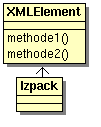
\includegraphics[width=0.15\textwidth]{../image/sol_casInitial.png}
	\hfil
	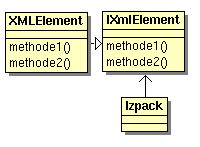
\includegraphics[width=0.3\textwidth]{../image/sol_extractionInterface.png}
	\caption{Extraction de l'interface}
\end{figure}
Nous avons ensuite créé l'implémentation de l'adaptateur respectant l'interface.
Izpack utilise alors la même interface mais notre implémentation était utilisé.
\begin{figure}[H]
	\centering
	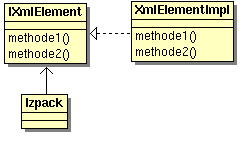
\includegraphics[width=0.4\textwidth]{../image/sol_implementation.png}
	\caption{Implémentation de l'adaptateur}
\end{figure}
Il suffit alors de supprimer NanoXml, ses utilisations ayant été remplacés par notre implémentation.
\subsection{Implémentation de Xinclude}
Avec NanoXml, la balise \verb|xinclude| permet d'inclure un fichier xml externe.
Ainsi, on peut utiliser un xml très succinct (et donc facilement lisible/compréhensible) qui inclut d'autres fichiers xml décrivant uniquement certaines parties de l'installation.
Cette fonctionnalité, absente de nanoXML, avait été mise en place en modifiant directement le code de son parseur.

Xinclude est présente dans les normes W3C et Jaxp l'intègre dans son implémentation.
Pour que Jaxp prenne en compte les balises Xinclude, il faut que le parser prenne en compte les espaces de nommage (namespaces) XML.
En effet, le Xinclude appartient au namespace \verb|xi|.
Il faut donc utiliser la balise \verb|<xi:include/>| au lieu de \verb|<xinclude/>|.
Le simple fait de rendre le parser namepaceAware permet d'utiliser la fonctionnalité Xinclude.
\subsection{Implémentation de Xfragment}
La fonctionnalité Xfragment permet principalement d'ajouter des éléments sans racines avec Xinclude.
C'est à dire qu'au contenu du xml à ajouter, on va retirer les noeuds \verb|<xfragment>|.
Par exemple:
\begin{lstlisting}[language=xml]
<xfragment>
<root1>
	<noeud1>text</noeud1>
</root1>
<root2>
	<noeud1>text</noeud1>
</root2>
</xfragment>
\end{lstlisting}
Si ce xml est inclus, 2 éléments, \verb|<root1>| et \verb|<root2>| seront ajouté à l'emplacement du Xinclude.
Sans le xfragment, le Xml ne serait pas valide (plusieurs éléments racine) et il y aurait erreur au moment du parse.
Le Xfragment agit ici comme conteneur temporaire d'éléments.

Cette fonctionnalité a été rajouté a NanoXml et il était nécessaire de la conserver.
Cependant, elle ne fait pas partie des spécifications W3C et le parseur n'offre pas de base cette fonctionnalité.
Il a fallut trouver une solution pour implémenter cette fonctionnalité.
\subsubsection{Première solution, manipulation du DOM}
Une première solution est de modifier le DOM obtenu après le parse du XML. 
Il faudrait chercher les noeuds nommer Xfragment et les supprimer.
Cependant, la suppression d'un noeud en DOM entraîne la suppression de tout les éléments qu'il contient.
Il faudrait donc au préalable sauvegarder le contenu, supprimer l'élément et restaurer le contenu sauvegardé.
\subsubsection{Deuxième solution, surcharge du parseur}
Une autre solution est de procéder de la même manière que pour ce qui a été fait pour NanoXml.
C'est à dire de modifier le parseur pour traiter les xfragment de manière spécifique.
Cependant, cette solution, possible sous NanoXml, est difficilement réalisable sur Jaxp. 
En effet, les appels du parseur sont transmis vers des classes internes et difficilement manipulables.
\subsubsection{Troisième solution, transformation XSL}
La troisième solution a été proposé par Matthew Fudge, la personne ayant rajouté la gestion des Xfragment et Xinclude dans NanoXml pour IzPack.
Elle consiste à transformer l'arbre xml obtenu après le parse grâce à une transformation XSL (Extensible Stylesheet Language).
Les transformations XSL permettent de définir des règles de modification d'un XML et se présente lui-même sous la forme d'un XML.
Elles permettent de modifier facilement des XML de manière simple.
Elle convenait parfaitement à notre problème.
La feuille de style utilisé est la suivante :
\begin{lstlisting}[language=xml]
<xsl:stylesheet xmlns:xsl='http://www.w3.org/1999/XSL/Transform' version='1.0'>
    <xsl:template match="*">
        <xsl:copy>
            <xsl:copy-of select="@*"/>
            <xsl:apply-templates/>
        </xsl:copy>
    </xsl:template>
    <xsl:template match="xfragment">
        <xsl:apply-templates/>
    </xsl:template>
</xsl:stylesheet>
\end{lstlisting}
La règle appliquée sur un élément est la plus spécifique.
Ici, pour tout les éléments, on recopie l'élément.
Dans le cas du xfragment, on omet la copie.
Au final, le xfragment est supprimé du XML ce qui est le but recherché.
\subsection{Numéro de ligne}
Une fonctionnalité de nanoXML est la gestion des numéros de lignes. 
Lors qu'une incohérence est détectée dans un XML lu, IzPack prévient l'utilisateur de l'erreur, et indique le numéro de la ligne responsable dans le xml.

Du point de vue de DOM, les numéros de lignes n'ont pas de signification : une fois le fichier XML parsé, seul l'arbre DOM construit en mémoire importe. 
Cet arbre, réécrit dans un fichier ne correspondra pas forcèment (pour les numéros de lignes, l'indentation, etc) au fichier de départ, sans parler des ajouts/suppressions/modifications de noeuds.

Au contraire, pour SAX, les numéros de lignes sont obtenues facilement.
Dans ce cas là, il est utile de savoir à quel endroit on se trouve dans le document.

Afin d'obtenir les numéros de ligne dans un arbre DOM, les deux points de vue ont été utilisés grâce à un \verb|Transformer|.
Cet objet permet (entre autre) d'utiliser un parser SAX pour remplir un arbre DOM.
Lors du parse SAX on retient les numéros de lignes, qui seront ajoutés aux bons éléments du DOM.
Ce nombre est stocké dans les ``user data'', ajoutés dans la version 3  de DOM pour stocker diverses informations supplémentaires dans un noeud.

\section{Application et tests}
Une fois la solution réalisée, nous l'avons soumis à un certain nombre de tests afin de la vérifier.
\subsection{Tests}
Afin d'avoir un comportement le plus fidèle possible à celui de NanoXML et assurer la fiabilité de la solution, de nombreux tests unitaires ont été écrits.
\subsubsection{Test unitaires de comparaison}
La solution a d'abord été élaborée de manière isolée.
Un projet indépendant contenant NanoXml à été créé. 
C'est sur ce projet que nous avons travaillé et développer notre adaptateur.
Nous avons alors réalisé une batterie de tests couvrant toutes les méthodes de l'interface extraites et de très nombreux cas.
Ces tests unitaires effectuent des actions identiques avec notre adaptateur et NanoXML, et comparent les résultats.

Prenons l'exemple de la méthode \verb|getName()|. Le même fichier Xml est parsé par les 2 librairies.
Un parcours récursif de l'arbre XML est effectué sur les 2 arbres en mémoire.
Pour chaque élément, on compare le résultat de la méthode \verb|getName()| sur l'élément courant : les retours doivent être toujours égaux.

Comme les méthodes de XMLElement sont souvent des récupérations d'informations de la même nature que getName(), nous avons généralisé ce test à ces méthodes.
Pour cela, une méthode se charge de parcourir de manière récursive l'arbre et d'invoquer la méthode à tester en comparant leurs résultats.
Ceci nous a permis de nous assurer du comportement de l'adaptateur et de déceler des anomalies sur NanoXml.

En couvrant la quasi totalité des méthodes utilisées dans IzPack avec de nombreux cas d'utilisation, nous avons pu nous assurer du respect du comportement de notre adaptateur.
\subsubsection{Les tests unitaires sur Xinclude et Xfragment}
Avec l'ajout des fonctionnalités XInclude et XFragment à NanoXml, une batterie de test unitaires a été fournies.
Nous avons donc repris ces tests et nous les avons intégrés aux tests de l'adaptateur.
\subsubsection{Les tests unitaires classiques}
Nous avons créé une batterie de tests unitaires classiques pour notre adaptateur.
Ils s'assurent entre autre que le parse, l'exploitation de l'arbre en mémoire et l'écriture du Xml se font correctement.
\subsection{Intégration a IzPack}
L'intégration à IzPack de notre travail fut relativement aisée : les objets de NanoXml ont été remplacés par ceux de notre adapteur.
Les appels n'ont quasiment pas été changés, les méthodes exposées dans les deux cas étant les mêmes.
Cette intégration effectuée, nous avons pu commencer les tests sur application.
\subsubsection{Test fonctionnels}
Une phase de test fonctionnels a été réalisée pour tester l'intégrité de l'application après l'intégration de notre solution.
Ces tests sont des tests manuels sur les installations générés par Izpack.
Nous avons donc testé dans un premier temps l'application d'exemple fourni par Izpack.
Ces tests ont permis de faire ressortir quelques problèmes que nous avons pu régler rapidement.

Suite à cela, nous avons essayé de générer et lancer un installeur plus conséquent.
Nous avons pour cela utilisé l'installeur de Glassfish.
La génération et l'installation de glassfish s'est déroulé sans problème.
\subsubsection{Profiling}
Après la phase d'implémentation et de test, nous avons pu commencer une phase d'optimisation.
En utilisant YourKit, nous avons essayé de détecter les méthodes chronophages lors d'une installation et les modifier éventuellement.

\section{Résultats}
Le principal but de notre projet a été de pouvoir abandonner NanoXml ce qui est chose faite.
De plus, l'intégration de notre solution a apporté un certain nombres d'avantages.
\subsection{Diminution de la taille des installeurs}
Tout d'abord, l'abandon de NanoXml diminue la taille de IzPack et des installeurs générés car cette librairie n'a plus besoin d'être présente dans les installeurs.
NanoXml pèse, une fois compilé, 116Ko.
Notre adaptateur pèse 44Ko.
Chaque installeur généré par Izpack perdra donc 72Ko.
Ce chiffre peut paraître faible mais si l'installeur est téléchargé 25000 fois sur le site officiel, presque 1800 Mo de bande passante sont économisés.
\subsection{Support de fonctionnalités XML}
Outre le fait d'avoir un parseur plus fiable et récent, un certain nombre de nouveautés ont été apportées.
\subsubsection{Support de la DTD}
Désormais les DTD (document de validation d'un xml) sont pris en charge.
\subsubsection{Support natif de Xinclude}
De plus, l'inclusion de fichiers xml dans d'autres est supporté nativement, sans avoir à modifier le code du parseur.
\subsection{Intégration dans la branche principale}
Régulièrement, nous synchronisions notre dépôt avec la branche principale pour prendre en compte les modifications qui ont été réalisées sur Izpack.
Cette synchronisation se passait généralement sans encombre grâce à Git, excepté quand les modifications concernaient la manipulation de XML et que les fichiers étaient conséquents (>3000 lignes).

Cette synchronisation régulière était en vue de préparer le merge vers sur la branche principale.
Ainsi, une fois notre solution achevée et testée, Julien Ponge a extrait un patch qui a été soumis à la communauté des développeurs d'Izpack.
Après quoi, les modifications ont été portées sur la branche principale et seront disponibles pour la prochaines version d'Izpack, la 4.3.
\section{Au delà du sujet}
Une fois l'objectif du projet atteint, nous avons décidé d'accepter l'offre de Julien Ponge en devenant contributeurs officiels du projet.
\subsection{Le projet Izpack}
Izpack est une communauté Open-Source, sa structure et son fonctionnement sont particuliers. 
Le projet est récemment passé sous CodeHaus. 
Des outils et des moyens de communications sont dédiées au projet.
\subsubsection{Codehaus}
CodeHaus est une fondation dédiée au développement de projets open-source.
A ce titre, elle propose une plateforme pour aider au développement de ces projets avec un certains nombre d'outils fournis par des sponsors.
Par exemple, Atlassian fournit pour les projets leur système de suivie de bug, JIRA, JetBrain fournit une licence IntelliJ, etc...
\subsubsection{Structure de la communauté}
Les projets sous CodeHaus sont des méritocraties. 
Un despote supervise un projet.
Les développeurs désirant rejoindre un projet doivent apporter une contribution, montrer leur motivation et être approuvés par le despote.
En général, les décisions se prennent de manière démocratiques pour tout ce qui concernent le projet.

Une mailing-list pour les développeurs permet de communiquer les informations et prendre les décisions d'un commun accord.
Pour éviter tout blocage dans les décisions, le despote a toujours le dernier mot.

Dans le cas de Izpack, le despote est Julien Ponge.
\subsubsection{Système de suivi de bugs, Jira}
L'évolution du projet peut être suivie via Jira.
Les anomalies, lacunes et améliorations possibles font l'objet d'un ticket.
Jira permet alors de suivre et de modifier les tickets avec un workflow similaire à LightHouse.
\begin{figure}[H]
	\centering
	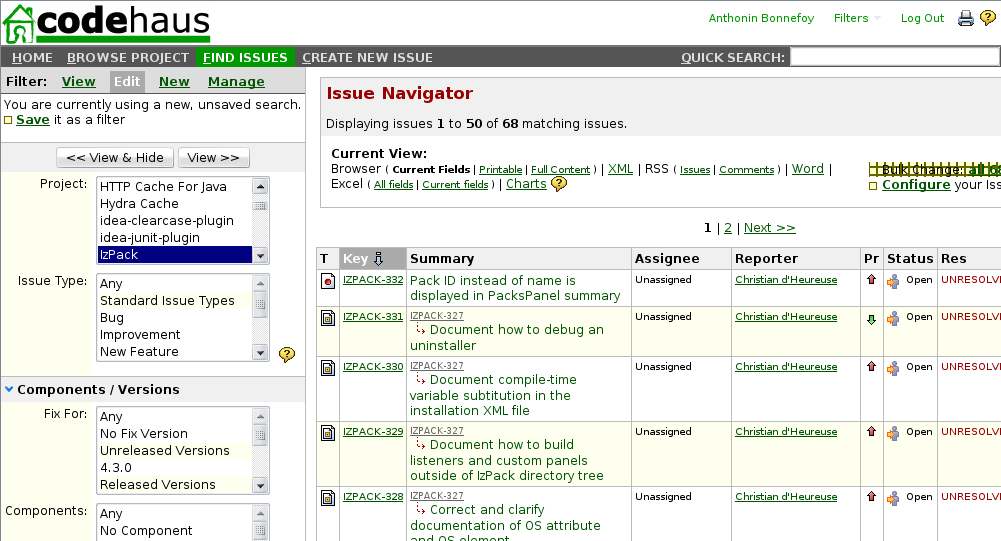
\includegraphics[width=0.8\textwidth]{../image/jira.png}
	\caption{Dashboard Jira}
\end{figure}
\subsection{Suivi de nos apports}
Notre solution étant intégrée, il est possible que des bugs subsistent dans notre implémentation ou qu'une mauvaise interprétation de notre part mène à un comportement inattendu.
Le statut de développeur nous permet de suivre et corriger les problèmes rencontrés par la communauté de IzPack.
\subsubsection{Tests corrigés}
Nous avons par exemple corrigé des tests unitaires sur les numéros de ligne échouant et sur les conditionsTest.
\subsubsection{Rectification sur une interprétation}
Un problème est apparu lors de l'utilisation du Xinclude.
Ce problème a été notifié par un développeur utilisant la version de développement et donc ayant récupéré nos modifications.

Par défaut, Jaxp résout le chemin de manière relative au répertoire d'exécution et c'est ce qui a été réalisée dans notre implementation.
Or le comportement attendu, plus naturel, est de résoudre le chemin d'inclusion relativement au document incluant le xml.

\subsection{Correction de bugs}
Nous avons également corrigé plusieurs bugs.
\subsubsection{Problème lors de l'installation automatique}
Un panel, le TreePacksPanels, ne respectait pas la configuration enregistrée lors de l'installation normale. 
Le problème provenait d'un problème de packaging, la classe devant faire le travail automatique n'était pas présente lors de l'installation.

Un bug caché dans l'installation automatique pouvait la faire quitter silencieusement.
\subsubsection{Web installers}
Izpack possède une fonction de création d'installeurs Web.
Cette fonctionnalité permet de générer des modules d'installations qui pourront être déposés sur un serveur web avec un installeur léger contenant uniquement le noyau dur.
Les modules additionnels seront alors téléchargés s'ils sont sélectionnés.

Cette fonctionnalité présentait des lacunes dans la documentation et n'était pas fonctionnelle.
De plus, un refactoring des classes concernés est en cours de traitement.
\subsubsection{UserInputPanels}
Le panel UserInputPanels doit permettre de décider de l'alignement des éléments.
C'est a dire qu'il est possible de les placer à gauche, à droite ou au centre. Actuellement, tout les éléments sont alignés à gauche.
Le travail est en cours de réalisation mais les modifications entrent en concurrence avec le refactoring de Dennis Reil, un autre contributeur.

\subsection{Améliorations}
Outre les corrections de bugs, la qualité du code a été également amélioré.
Par exemple, le code de l'installeur automatique a été refactoré avec d'autres classes, rendant le code plus lisible et améliorant sa qualité.

De même, certaines méthodes inutilisées (prévues pour des vieilles versions de java) ont pu être supprimées.